\documentclass[conference]{IEEEtran}
\IEEEoverridecommandlockouts
% The preceding line is only needed to identify funding in the first footnote. If that is unneeded, please comment it out.
\usepackage{cite}
\usepackage{textcomp}
\usepackage[dvipsnames, table]{xcolor}


\usepackage{booktabs,multirow,array,hhline}
\newcolumntype{N}{@{}m{0pt}@{}}
%\usepackage[margin=15mm]{geometry}
\usepackage{amsmath}
\usepackage{amssymb}
\usepackage{bm}
\usepackage{amsfonts}
\usepackage{tikz}
\usepackage{mathdots}
\usepackage{cancel}
\usepackage{color}
\usepackage{siunitx}
\usepackage{array}
\usepackage{multirow}
\usepackage{gensymb}
\usepackage{tabularx}
\usepackage{booktabs}
\usetikzlibrary{fadings}
\usetikzlibrary{patterns}
\usetikzlibrary{shadows.blur}
\usepackage{booktabs} % For formal tables
\usepackage{graphicx}
\usepackage{mathtools}
\usepackage{subcaption}
\usepackage{xspace}
% \captionsetup{compatibility=false}
\usepackage[ruled,vlined, linesnumbered]{algorithm2e}
\usepackage{import}
\usepackage{url}
\usepackage{enumitem}
\usepackage{comment}

% table and siunits
\usepackage{tabularx, siunitx}
\newcommand{\best}{{\cellcolor[gray]{0.75}}}
\newcommand{\statsimilar}{{\cellcolor[gray]{0.9}}}
\newcommand{\algremark}[1]{\tcc*[r]{#1}}
\newcommand{\iqr}{{\small}}

\usepackage[noend]{algpseudocode}
\makeatletter
\def\BState{\State\hskip-\ALG@thistlm}
\makeatother


%% MATHS COMMANDS
% for algorithms
\DeclarePairedDelimiter\abs{\lvert}{\rvert}%
\newcommand{\lcbucbscalar}{k\xspace}
\newcommand{\evaluatedx}{\bX}
\newcommand{\paretofront}{\mathcal{F}}
\newcommand{\paretoset}{\mathcal{P}}
\newcommand{\predict}{\hat{f}}
\newcommand{\attainmentfront}{\mathcal{A}}
\newcommand{\attainmentset}{\evaluatedx_{\mathcal{A}}}
\newcommand{\ninitialevaluations}{N}
\newcommand{\nevaluations}{t}
\newcommand{\nbudget}{B}
\newcommand{\parameterspace}{\mathcal{X}}
\newcommand{\ndim}{d}
\newcommand{\nobj}{M}
\newcommand{\rp}{\mathbf{R}}
\newcommand{\defn}{\triangleq}

\DeclareMathOperator*{\sig}{sig}
\DeclareMathOperator*{\saf}{SAF}
\DeclareMathOperator*{\msafmu}{SAF_\mu}
\DeclareMathOperator*{\OSAF}{osaf}
\DeclareMathOperator*{\DSAF}{dsaf}
\DeclareMathOperator*{\MMIN}{maximin}
\DeclareMathOperator*{\MMAX}{minimax}
\DeclareMathOperator*{\mgp}{\mathcal{GP}}


\DeclareMathOperator*{\union}{\medcup}
\DeclareMathOperator*{\argmax}{\arg\!\max}
\DeclareMathOperator*{\argmin}{\arg\!\min}
\DeclareMathOperator*{\bigO}{\mathcal{O}}
\DeclareMathOperator*{\erf}{\text{erf}}
\DeclareMathOperator*{\cov}{\text{cov}}
\DeclareMathOperator{\diag}{diag}
\DeclareMathOperator{\nondom}{nondom}
\DeclareMathOperator{\LatinHypercubeSampling}{LHS}
\DeclareMathOperator{\posterioruncertainty}{\bm{\sigma}}


\DeclareMathOperator*{\igdp}{IGD^{+}}
\newcommand\hpv{dominated hypervolume\xspace}
\newcommand\safmu{SAF$_{\mu}$\xspace}
\newcommand\safei{SAF$_{EI}$\xspace}
\newcommand\smsego{SMS-EGO\xspace}
\newcommand\smsegomu{SMS-EGO$_{\mu}$\xspace}
\newcommand\parego{ParEGO\xspace}
\newcommand\mpoi{MPoI\xspace}
\newcommand\ei{EI\xspace}
\newcommand\gp{GP\xspace}
\newcommand\gps{GPs\xspace}
\newcommand\maximin{maximin\xspace}
\newcommand\lhs{LHS\xspace}
\newcommand\igd{IGD$^+$\xspace}

\newcommand\target{\mathcal{T}}
\newcommand\mF{\mathcal{F}}
\newcommand\mP{\mathcal{P}}
\newcommand\Papprox{\tilde{\mathcal{P}}}
\newcommand\Fapprox{\tilde{\mathcal{F}}}
\newcommand\mGP{\ensuremath{\mathcal{GP}}\xspace}
\newcommand\mD{\mathcal{D}}
\newcommand\mN{\mathcal{N}}
\newcommand\mX{\mathcal{X}}
\newcommand\normal{\mathcal{N}}
\newcommand{\inv}{^{-1}}
\newcommand\natnum{\mathbb{N}}
\newcommand\expc{\mathbb{E}}
\newcommand*{\medcup}{\mathbin{\scalebox{1.5}{\ensuremath{\cup}}}}
\newcommand{\reals}{\mathbb{R}}
\newcommand{\trp}{^\top}
\newcommand{\given}{\,|\,}



\newcommand{\pigdref}{\mathcal{Z}}
\newcommand{\bx}{\mathbf{x}}
\newcommand{\bu}{\mathbf{u}}
\newcommand{\bv}{\mathbf{v}}
\newcommand{\bX}{\mathbf{X}}
\newcommand{\by}{\mathbf{y}}
\newcommand{\bI}{\mathbf{I}}
\newcommand{\bz}{\mathbf{z}}
\newcommand{\brr}{\mathbf{r}}
\newcommand{\bff}{\mathbf{f}}
\newcommand{\bF}{\mathbf{F}}
\newcommand{\bzero}{\mathbf{0}}
\newcommand{\bmu}{\boldsymbol{\mu}}
\newcommand{\bphi}{\boldsymbol{\phi}}
\newcommand{\fhat}{\hat{f}}
\newcommand{\fstar}{f^\star}
\newcommand{\xnext}{\bx'}
\newcommand{\data}{\mathcal{D}}
\newcommand{\FIXME}[1]{[\textcolor{red}{\textbf{FIXME} \textsl{#1}]}}
\newcommand{\rmenote}[2][\textcolor{magenta}{\dagger}]{$#1$\marginpar{\color{magenta}\raggedright\tiny$#1$ #2}}
\newcommand{\mnote}[2][\textcolor{red}{\dagger}]{$#1$\marginpar{\color{red}\raggedright\tiny$#1$
    #2}}
\newcommand{\fnote}[2][\textcolor{teal}{\dagger}]{$#1$\marginpar{\color{teal}\raggedright\tiny$#1$
    #2}}
\newcommand{\mnotejf}[2][\textcolor{blue}{\dagger}]{$#1$\marginpar{\color{blue}\raggedright\tiny$#1$ #2}}

\newcommand*{\eg}{e.g.\@\xspace}
\newcommand*{\ie}{i.e.\@\xspace}
\newcommand*{\etal}{\textit{et al.}\@\xspace}

\begin{document}

%
\title{Multi-objective Bayesian optimisation using an exploitative  attainment front acquisition function}

%Exploitative and Bayesian multi-objective optimisation: a summary attainment front acquisition function
%

\author{
  \IEEEauthorblockN{Finley J. Gibson}
  \IEEEauthorblockA{\textit{Department of Computer Science,}\\
      \textit{University of Exeter,}\\
      Exeter, UK\\
      \url{F.J.Gibson@exeter.ac.uk}
      }
      \and
       \IEEEauthorblockN{Richard M. Everson}
  \IEEEauthorblockA{\textit{Department of Computer Science,}\\
      \textit{University of Exeter,}\\
      Exeter, UK\\
      \url{R.M.Everson@exeter.ac.uk}
      }
      \and
       \IEEEauthorblockN{Jonathan E. Fieldsend}
       \IEEEauthorblockA{\textit{Department of Computer Science,}\\
      \textit{University of Exeter,}\\
      Exeter, UK\\
      \url{J.E.Fieldsend@exeter.ac.uk}
    }
  }

  \maketitle

\begin{abstract}

    %Efficient methods for optimising expensive black-box problems with multiple objectives can often themselves become prohibitively expensive as the number of objectives is increased. We propose an approach to efficient optimisation of such problems without the reliance on hypervolume and expected improvement computation, which are the principal causes of poor dimensional scaling in current state-of-the-art  approaches.  We show that our approach is able deliver similar performance to the current state-of-the-art, and further show that approaches based on surrogate mean predictions are superior to the widely used \textit{expected improvement} when\mnote{with?} the Gaussian process surrogate models, typically applied. Performance is evaluated on the well-known Walking Fish Group problem set, against current state-of-the art approaches. 
 
    Efficient methods for optimising expensive black-box problems with multiple objectives can often themselves become prohibitively expensive as the number of objectives is increased. We propose an infill criterion based on the distance to the summary attainment front which does not rely on the expensive hypervolume or expected improvement computations, which are the principal causes of poor dimensional scaling in current state-of-the-art approaches. By evaluating performance on the well-known Walking Fish Group problem set, we show that our method  delivers similar performance to the current state-of-the-art.  We further show that methods based on surrogate mean predictions are more often than not superior to the widely used expected improvement, suggesting that the additional exploration produced by accounting for the uncertainty in the surrogate's prediction of the optimisation landscape is often unnecessary and does not aid convergence towards the Pareto front. 

\end{abstract}


\begin{IEEEkeywords}
Expensive optimisation, Bayesian optimisation, infill criteria, acquisition functions.
\end{IEEEkeywords}


\section{Introduction}
The process of optimising black-box functions relies exclusively on querying the underlying objective function in order to advance the understanding of the parameter objective-space mapping of, and convergence toward, an optimal solution. During the optimisation process a balance must be struck between the exploitation of the function as currently understood in order to find good solutions, and further exploration of the unknown regions of its landscape in order to advance this understanding. Extensive work has gone into theorising how this balance should be managed, particularly in cases where there is a high cost associated with querying the underlying objective. Careful management of this balance is considered essential if a suitable solution is to be found as efficiently as possible. Bayesian optimisation \cite{jones1998efficient}, which constructs a probabilistic surrogate model of the objective function, has emerged as an effective means of solving such problems, and has been widely applied to many problems with success.

In the field of multi-objective optimisation (MO), accurately modelling the multi-dimensional objective function is more challenging, as many techniques used in single-objective optimisation require (hyper-) volume measurements and integration, which are complex in higher dimensions. One widely used technique is to calculate and the expected improvement (\ei) \cite{jones1998efficient} in the dominated hypervolume to manage the exploitation/exploration trade-off. However, recent work has shown that in single objective problems with high-dimensional parameter spaces, the low fidelity between the commonly used surrogate models and the underlying function reduces the need to actively explore the function. Instead purely exploitative methods have been demonstrated to outperform methods which balance the explore/exploit trade-off \cite{death2019greed}. With this in mind we investigate the use of exploitative approaches in the multi-objective domain, anticipating the increased complexity of modelling problems with multi-dimensional outputs will similarly benefit from exploitative methods. 

We are concerned with multi-objective problems (MOPs) for which the cost associated with the evaluation of the objectives for a set of parameters is significant, which heavily restricts the evaluation budget during an  optimisation. This can be because either each objective is independently expensive and requires a separate evaluation or, more commonly, all objectives are jointly evaluated by a single expensive process. In such MOPs the goal of the optimisation process is to find a suitable solution in as few evaluations of the objective function(s) as possible.  Large-scale simulation and embodied optimisation, requiring physical intervention for objective evaluation, has emphasised the importance of these expensive problems \cite{osio1996engineering,  li2017rapid, jeong2005efficient, fang2017design, huband2005scalable} as more traditional multi-objective evolutionary algorithms require prohibitively large numbers of evaluations. 
%\rmenote{Could give some more references to work in this area if room} 
%This class of problem is common in real-world applications, particularly in the fields of engineering and computer modelling. For example, when engineering a component based on some design parameters, performance evaluation of a newly proposed design may require making and testing the component, incurring both time and material costs \cite{fang2017design}. Alternatively, computationally expensive processes such as fluid dynamic simulation or machine learning model evaluation, often have high computational costs associated with them and can take hours or even days to process \cite{huband2005scalable}. This renders optimiser classes such as Multi-Objective Evolutionary Algorithms\cite{tanabe2017benchmarking,coello2007evolutionary,tamaki1996multi}, for which a large number of objective evaluations are required, unsuitable.

In this paper we explore the use of a cheap to compute minimax infill criterion to avoid the expensive dominated hypervolume calculation.  We also investigate whether incorporating the surrogate model uncertainty is effective, finding that in fact an exploitative approach is at least as effective and computationally cheaper. The principal contributions of this work are:
\begin{itemize}[left=0pt .. \parindent]
    \item We propose a novel, cheap to compute, infill criterion for evaluating the suitability of candidate parameters at  which to next evaluate the true objective function, %\mnotejf{surely it is the efficacy of the design, not the objective vector of the design?}
    based on the distance to the summary attainment front (SAF). 
    \item We give an extensive empirical evaluation of the Walking Fish Group problem set \cite{huband2005scalable} and show that the SAF infill criterion yields state-of-the-art performance in Bayesian multi-objective optimisation, equalling or surpassing the current leading methods, with lower computational complexity. 
    \item We show empirically that exploiting the mean prediction of the surrogate model is  usually superior to deliberately exploring regions of uncertainty in the surrogate posterior prediction.  
\end{itemize}

In the following section we summarise the Bayesian optimisation approach, particularly in the multi-objective context and discuss works related to this topic.  Then in section \ref{section:our_method} we describe the novel SAF infill criterion, and describe the optimisation process used.  The experimental evaluation process is described and findings discussed in section \ref{section:our_method}.


\section{Background}
\subsection{Bayesian Optimisation}\label{section:background_BayesianOptimisation}
Bayesian optimisation (BO) is a form of efficient global optimisation (EGO), which searches for the global optimal solution to an objective function $f(\mathbf{x})$ for  $f: \parameterspace \subset \mathbb{R}^{\ndim} \mapsto \mathbb{R}$\fnote{is this okay? Do i need to mention $\bx \in \parameterspace$?}, while making as few evaluations of the objective function as possible. In BO, in order to limit the number of evaluations required of the true objective function,  a small number of $\ninitialevaluations$ initial evaluations are made, and a probabilistic surrogate model is then generated from these evaluations. This surrogate model, which should be cheap to evaluate, can then be used to predict the quality of subsequent candidate solutions without the need to frequently evaluate $f$.   Unlike other surrogate modelling methods, BO constructs a probabilistic surrogate model which allows the model's uncertainty as well as its mean predication to be accounted when choosing the next location for evaluation.

% \begin{algorithm}[t]
%   \SetAlgoLined
%   \KwResult{minimiser of $f(\bx)$}
%   \SetKwInOut{Input}{Input}
%   \SetKwInOut{Output}{Output}
%   \SetKwComment{tcc}{}{}
%   \SetCommentSty{textit}
%   \DontPrintSemicolon
%   \Input{$\ninitialevaluations$ - number of initial evaluations}
%   \Input{$\nbudget$ - evaluation budget}
%   \BlankLine
%   %\textbf{Initialization}
%   %\tcc*[l]{\textbf{Initialisation:}\hfill Generate initial samples}
%   $X \gets \text{LHS}(\parameterspace, \ninitialevaluations)$ \label{alg: BO_LHS}
%   \algremark{Generate initial samples}
%   \For {$t = 1 \xrightarrow{} \ninitialevaluations$ \do}{ \label{alg:initial-start}
%     $f_t \gets f(\bx_t)$ \algremark{Expensively evaluate initial samples}
%     } \label{alg:initial-end}
%   $\data  \gets \{(\bx_t, f_t)\}_{t=1}^{\ninitialevaluations}$
%   \BlankLine 

%   \For{$t = \ninitialevaluations+1\xrightarrow{}\nbudget$ \do}{
%   $ \theta \gets \text{train} \;\mathcal{GP}(\data)$ \label{alg:train}\\
%   $\bx_t \gets \underset{\mathbf{x}\in \parameterspace}{\argmax} \:
%   \alpha(\mathbf{x}; \theta)$ \label{alg:opt-alpha} \algremark{Maximise acquisition fcn}
%   $ f_t \gets f(\bx_t)$ \label{alg:expensive} \algremark{Expensively evaluate $\bx_t$}
%   $\data \gets \data \cup \{(\bx_t, f_t)\}$ \algremark{Augment data}}
%   %\Output{$\bx_t \quad \quad \underset{t\in 1:\nbudget}{\argmin} f_{1:\nbudget}$}
%   \Output{$ \argmin_{\bx_t\in \data} \{f(\bx_t)\}$}
% \caption{Bayesian optimisation}
% \label{alg:BO}
% \end{algorithm}

The process of BO %, summarised in Algorithm \ref{alg:BO},
involves first selecting a set of $\ninitialevaluations$ initial candidate solutions, usually via Latin hypercube sampling (LHS) \cite{mckay2000comparison}, and evaluating the objective function for each of these to produce a set $\mathcal{D} = \{ (\bx_t, f_t \triangleq f(\bx_t) )\}_{t=1}^{\ninitialevaluations}$.
% ; lines \ref{alg:initial-start}-\ref{alg:initial-end} in Algorithm \ref{alg:BO}. 
A probabilistic, surrogate model is then fitted to these observations, for which  Gaussian processes (\gp) are commonly used; see \cite{rasmussen2003gaussian} for a comprehensive introduction.
The \gp describes the current belief about the objective function, modelling it as a set of random variables with a joint Gaussian distribution.  The predictive probability distribution $\predict(\bx)$ at a location $\bx$ is a normal distribution:
\begin{equation}\label{eqn:predictive_probability_distribution}
P\big(\predict(\mathbf{x}) \given \mathbf{x}, \mathcal{D}, \theta \big) = 
\mathcal{N}\big(\bmu(\mathbf{x}), \sigma^2(\mathbf{x})\bI\big)
\end{equation}
where $\mu$ and $\sigma$ are mean and standard deviation predictions given by:
\begin{align}\label{eqn: mu}
\mu(\mathbf{x}) &= \boldsymbol{\kappa}(\mathbf{x}, \evaluatedx) - K^{-1}  \bphi,\\
\label{eqn: sigma}
\sigma^2(\mathbf{x}) &= \kappa(\mathbf{x}, \mathbf{x}) - \boldsymbol{\kappa}(\mathbf{x}, \evaluatedx)^{\top}K^{-1} \boldsymbol{\kappa}(\evaluatedx, \mathbf{x}).
\end{align}
Here $\evaluatedx$ is the $\ndim$ by $\nevaluations$ matrix of locations at which $f(\bx)$ has
been previously evaluated, $\bphi = (\bx_1, \bx_2, \ldots, \bx_{\nevaluations})$.
$\kappa(\mathbf{x}, \mathbf{x}')$ is a predefined
covariance function, or  \textit{kernel}, between $\mathbf{x}$ and
$\mathbf{x}'$, and  $K$ is the covariance matrix comprised of all
covariances $\kappa(\mathbf{x}, \mathbf{x}') \; \forall \: \mathbf{x},
\mathbf{x}'\in \evaluatedx$. A vector of the covariances between
$\mathbf{x}$ and each of the $t$ locations in $\evaluatedx$ is denoted
$\boldsymbol{\kappa}(\mathbf{x}, \evaluatedx)\in \mathbb{R}^{t}$. The vector of covariances between each of the $t$ locations in
$\evaluatedx$ and $\mathbf{x}$ is denoted $\boldsymbol{\kappa}(\evaluatedx,
\mathbf{x}) \in \mathbb{R}^{t}$. The parameters of the covariance function
(and any noise model) are denoted by $\theta$: these are learned on receipt of each new $(\bx, f(\bx))$ pair by maximising the likelihood of the data \cite{rasmussen2003gaussian}. 
% ; Algorithm \ref{alg:BO} line \ref{alg:train}. 


Determination of how desirable a new evaluation of the objective function
would be at a new location is achieved via an acquisition function $\alpha(\mathbf{x};  \theta)$, which balances the exploitation of locations predicted by the surrogate (with parameters $\theta$) to be good with high confidence, with the exploration of regions that have high uncertainty and might therefore contain the optimum. Maximisation of the acquisition function 
%(Algorithm \ref{alg:BO} line \ref{alg:opt-alpha}) 
yields the next location $\bx'$ at which to evaluate the real objective function: 
\begin{equation}\label{eqn: argmax_alpha}
   \bx' = \underset{\mathbf{x} \in \parameterspace}{\argmax}\:\alpha(\mathbf{x};  \theta).
 \end{equation}
A widely used acquisition function is the Expected Improvement
\cite{jones1998efficient}.  Here the improvement of a value $f$, over the best solution
evaluated so far, $f^\star = \min \{f(\bx_i)\}_{i=1}^t$ is $I(\bx,
 f^\star) = \max(f^\star -f, 0)$.  The expected improvement at $\bx$ on the basis of
the model is therefore
  \begin{align}
   \label{eq:EI}
    \alpha(\bx, f^\star) &= \int_{-\infty}^\infty  I(\bx, f^\star) p(f \given \bx, \data)\,df \\
   &= \sigma(\bx) \left( s\Phi( s) - \phi (s)\right) \label{eq:ei-closed-form}
  \end{align}
 where $s = (f^* - \mu(\bx)) / \sigma(\bx)$, and $\phi(\cdot)$ and
 $\Phi(\cdot)$ are the Gaussian probability density function and cumulative
 density functions. This acquisition function is essentially the improvement
 weighted by the part of the posterior predictive distribution that lies
 below the evaluated minimum $f^*$ and thus balances the exploitation of
 solutions which are very likely to be a little better than $f^*$ with the
 exploration of others which may, with lower probability, turn out to be
 much better. Other acquisition functions, which achieve the
 exploration-exploitation balance in different ways include the probability
 of improvement (PI) \cite{kushner:ego}, optimistic strategies such as UCB
 \cite{srinivas:ucb:2010}, expected improvement \cite{jones1998efficient},
 $\epsilon$-greedy strategies \cite{bull2011convergence, death2019greed},
 and information-theoretic approaches, e.g. \cite{scott:kg:2011,
   ru:fitbo:2018}.  Under certain conditions \ei and UCB have been shown to converge
\cite{bull2011convergence, srinivas:ucb:2010}.


\begin{comment}
 Commonly acquisition functions leverage the uncertainty in the posterior prediction to balance exploitation and exploration of the objective function. This is sometimes done by applying some some scalar $\lcbucbscalar$ to balance exploration, either in computation of the upper confidence bound (UCB) or lower confidence bound(LCB \cite{srinivas:ucb:2010}:
 \begin{align}
  \label{eq:UCB}
    \alpha_{UCB}(\bx, \theta) &= \mu(\bx) + \lcbucbscalar \sigma(\bx)\\
    \alpha_{LCB}(\bx, \theta) &= \mu(\bx) - \lcbucbscalar \sigma(\bx)
\end{align}
More commonly a computation of the probability of improvement (POI)  \cite{kushner:ego} is used, where integration of \eqref{eqn:predictive_probability_distribution} between infinity and the current best solution evaluated so far, $f^\star = \min \{f(\bx_i)\}_{i=1}^t$ gives the cumulative distribution of \eqref{eqn:predictive_probability_distribution} which improves on $\fstar$ and thus the probability of a sample drawn from \eqref{eqn:predictive_probability_distribution} yielding improvement\fnote{Am I okay to give $\fstar$ as an argument here? given that just $\theta$ is shown previously?}:

 \begin{align}
  \label{eq:POI}
    \alpha_{POI}(\bx, \theta, \fstar) &= \Phi \Bigg( \frac{\mu(\bx)-\fstar}{\sigma(\bx)} \Bigg)
\end{align}
 
 Incorporating the \textit{amount} of improvement associated with POI computation given by $I(\bx, \theta) = (\mu(\bx)-\fstar) \forall \mu(\bx)>\fstar$ and 0 otherwise, gives the \ei acquisition function \cite{jones1998efficient}. The expected improvement at $\bx$ on the basis of the model is therefore
 \begin{align}
  \label{eq:EI}
  \begin{split}
    \alpha_{EI}(\bx, \theta, \fstar) = (\mu(\bx)-\fstar)
    &\Phi \Bigg( \frac{\mu(\bx)-\fstar}{\sigma(\bx)} \Bigg) 
    +\\
    &\sigma(\bx)
    \phi \Bigg( \frac{\mu(\bx)-\fstar}{\sigma(\bx)} \Bigg)
    \end{split}
\end{align}
 where $\phi$ and $\Phi$ are the Gaussian probability density function and
 cumulative density functions. This acquisition function is essentially the
 probability of improvement weighted by the part of the posterior
 predictive distribution that is better than the evaluated $\fstar$ and
 thus balances the exploitation of solutions which are very likely to be a
 little better than $\fstar$ with the exploration of others which may, with
 lower probability, turn out to be much better.
\end{comment}


 Since evaluation of the acquisition function entails evaluating the model
 rather than $f$ itself, it can be  cheaply optimised using methods such as
 an evolutionary algorithm. 
%As shown in Algorithm \ref{alg:BO}, t
 This process of fitting a surrogate,
 and optimisation of the acquisition function and evaluation of $f$ is
 repeated, expanding $\mathcal{D}$, until a good solution is found and some
 stopping criteria is satisfied or the computational budget is exhausted.
 Since evaluation of the acquisition function entails evaluating the model
 rather than the objective function itself, it can be cheaply optimised
 using methods such as an evolutionary algorithm. 
 
 %As shown in Algorithm \ref{alg:BO}. This process of fitting a surrogate, optimising the acquisition function and evaluating $f$ at $\bx'$ is repeated, expanding the evaluated set $\mathcal{D}$, until a good solution is found and some stopping criteria is satisfied or the computational budget is exhausted.

\subsection{Multi-objective Bayesian Optimisation}\label{section:background_MOPs}
In MOPs, rather than a single criterion by which the success of a solution is assessed, a series of conflicting objectives is employed, between which some compromise must be reached. We denote the $\nobj$ conflicting objective functions by $f_m(\bx)$, $m = 1, \ldots, \nobj$, so that the MOP may be expressed 
as 
\begin{equation}\label{eqn: min_F}
\underset{\mathbf{x} \in \mX}{\argmin}\:\mathbf{f}(\mathbf{x}), 
\end{equation}
where $\parameterspace \subset \mathbb{R}^\ndim$ is the feasible space and and $\mathbf{f}: \parameterspace \mapsto \mathbb{R}^{\nobj}$.

A solution $\bx$ is said to dominate another $\bx'$ (denoted $\bx \prec \bx'$) if $f_i(\bx) \le f_i(\bx')$ for $i = 1, \ldots, \nobj$ and $ f_i(\bx) < f_i(\bx')$ for at least one $i$. Since in most cases with conflicting objectives there is no single dominating solution, the goal of most multi-objective optimisation algorithms is to produce a number of solutions which well represent the Pareto set, that is the maximal set of solutions that are not dominated by any other solutions in the feasible space:
\begin{equation}\label{eqn: Pareto_set}
  \paretoset = \{\mathbf{x} \in \parameterspace \;:\;
  \bx' \not\prec \bx \,\forall \bx' \in \parameterspace \}.
\end{equation}
%This is referred to as the summary attainment front (SAF),\mnote{no it is not -- you are confusing spaces and constructs here} and t
The image of $\paretoset$ under $\bff$ is the Pareto front, $\paretofront$. Since $\paretofront$ may contain infinitely many elements, usually  in multi-objective optimisation the best we can aspire to is an \emph{approximation} $\Papprox$, as represented by a set of mutually non-dominating solutions.   Given a set of solutions $\data$, we define the function $\nondom(\data)$ as the function that returns the non-dominated solutions in $\data$; thus $\Papprox = \nondom(\data)$.

% The $\nobj-1$ dimensional surface in objective space which separates the area/volume dominated by any element of this set from that which is non-dominated is known as the summary attainment front (SAF), hereby denoted $\attainmentfront$, and its parameters $\attainmentset$.
% \begin{equation}\label{eqn: Attainment_set}
%   \attainmentset = \{\mathbf{x} \in \evaluatedx \;:\;
%   \bx' \not\prec \bx \,\forall \bx' \in \evaluatedx \}.
% \end{equation}

% Multi-objective Bayesian optimisation is the extension of the process described in secion \ref{section:background_BayesianOptimisation} to the multi-objective setting in \ref{section:background_MOPs}.

Methods of Bayesian optimisation for MOPs generally fall into one of two
categories: single surrogate approaches and multi-surrogate approaches. The
mono-surrogate approach aggregates the $\nobj$ objective functions using a
scalarising function $g : \mathbb{R}^\nobj \mapsto \mathbb{R}$. Then using
$f(\bx) \defn g(\bff(\bx))$ the standard BO algorithm is used to optimise
$f$ and thus $\bff$. For example, the hypervolume improvement of a modelled
Pareto front over the current $\Papprox$ might be used as an
scalarising function. 



In a multi-surrogate approach, each objective $f_m$ is modelled
individually by its own separate surrogate which models
$P(f_m(\bx \given \data))$. These models are considered to be independent, thus ignoring cross-correlations between the models and the $P(f_m \given \bx, \data)$ are multiplied together to form the joint density $P(\bff \given \bx, \data) = \prod_{m=1}^\nobj P(f_m \given \bx, \data) $.
A scalarising function or infill criterion
$g : \mathbb{R}^\nobj \mapsto \mathbb{R}$ is used to evaluate the quality
of any modelled solution (for notational convenience and w.l.o.g.{} we assume that smaller $g$ means better solutions). Thus an expected improvement in $g(\cdot)$ may be found as:
\begin{align}
  \label{eq:EI-g}
    \alpha_{\ei}(\bx, g^\star) = \int_{-\infty}^\infty  \max(g(\bff(\bx) -
  g^\star, 0) P(\bff \given \bx,
  \data)\,d\bff
\end{align}
where $g^\star =  \min \{g(\bff(\bx_i))\}_{i=1}^t$.  Note that this
integral is multi-dimensional and, since it does not admit any closed form solution as in the single objective case \eqref{eq:EI},  must be
evaluated numerically, usually by Monte Carlo sampling from the distribution $P(\bff \given \data )$.

Practical experience shows that multi-surrogate methods tend to be superior to mono-surrogate approaches because a single \gp surrogate is unable to effectively model the highly complex function formed by the aggregated objectives, whereas each of the GPs in a multi-surrogate approach has the simpler task of modelling a single objective function \cite{rahat2017alternative}.   




% An acquisition function or infill criterion is then used to derive a scalar value which is maximised to find the next location to be expensively evaluated.  The alternative mono-surrogate approach is to use a surrogate to directly model the multivariate $\bff(\bx)$ from which the infill criterion is derived. 
% An acquisition function is then used to combine these distributions into a scalar quality measure:
% \begin{equation}\label{eqn: eqn: max_alpha_mop}
%    \bx' = \underset{\mathbf{x}\in \parameterspace}{\argmax}\:\alpha(\mathbf{x}; \{\theta_i\}_{i=1}^{\nobj})
% \end{equation}
% where $\theta_i$ denotes the parameters of the trained surrogate model of $f_i(\bx)$, and $g_i \mapsto \mathbb{R}$. In single surrogate models the $D$ objective functions are jointly modelled by a single function $g(\bx) \sim \bff(\bx)$, such that $g \mapsto \mathbb{R}^D$, and the $D$ dimensional vector $ \mathbf{g} \gets g(\bx)$ is combined into a scalar value by the acquisition function which is subsequently maximised to find the next location for expensive evaluation.
% \begin{equation}\label{eqn: eqn: max_alpha_monosurrogate}
%    \bx' = \underset{\mathbf{x}\in \parameterspace}{\argmax}\:\alpha(\mathbf{x}; \theta).
% \end{equation}

% Acquisition functions are more complex in MOPs than in single objective Bayesian optimisation, as the acquisition function must additionally combine the vector of surrogate predictions for each objective into a scalar value. Generalisations of \ei and PI to MOPs have been made by deploying mono-surrogates to jointly model the parameter space/objective space mapping, and then multi-dimensional integration is used to calculate the probability density function for a given set of parameters \cite{emmerich2006single,keane2006statistical}. The disadvantage of this is that multi-dimensional integration is computationally expensive and quickly becomes impractical due to the \textit{curse of dimensionality} associated with the dimensional increase resulting from the inclusion of additional objectives. More generally the acquisition function involves a function to interpolate between the explored points in the objective space, and then posterior predictions from the surrogate/surrogates are evaluated against this in order to quantify their suitability as candidates. 

\subsection{Related work}\label{section:related_work}

Bayesian approaches to solving MOPs tend to use Gaussian Process surrogates and largely differ in the acquisition functions by which parameters for the next objective function evaluations are selected. The acquisition functions which have proven most effective leverage measurement of the expected improvement to the \hpv, also known as the $\mathcal{S}$-metric  \cite{emmerich2008computation}, first suggested by Emmerich \etal \cite{emmerich2006single}.  The $\mathcal{S}$-metric improvement to the \hpv is the Heaviside difference between the \hpv  made over the estimated Pareto optimal solutions $\Papprox$ and the \hpv measurement over these solutions and the \gp model posterior prediction. For those locations which are not predicted by the model to improve the \hpv by some margin $\epsilon$, this is zero, and to these cases a penalty function is applied to overcome the resulting plateau in objective space. This penalty was originally calculated as the product of the $\nobj$ dimensional distances between the model prediction $\bff'(\bx)$ and each observation $p \in \Papprox$, summed over all elements of $\Papprox$,   but was later modified  to be the maximum of $\Papprox$ in order to reduce discontinuities in the resulting infill  \cite{wagner2010expected}. The resulting infill criterion for an $\nobj=2$ objective space is illustrated in Fig.\ \ref{fig: smsego_obj_space}. This approach naturally converges towards a set of solutions which well represent the Pareto front, as maximising the \hpv is equivalent to finding the true Pareto set \cite{fleischer2003measure}. 

The computation required to calculate the \hpv, and therefore the $\mathcal{S}$-metric, scales poorly with the number of objectives and the number of solutions forming $\Papprox$,  even the most efficient algorithms scaling as $O(|\Papprox|^D)$,  for $D \le 3$ and potentially worse beyond that \cite{hupkens2014faster}. Furthermore increasing $D$ results in larger $\Papprox$ because of the increasing proportion of objective space that is mutually non-dominating. 
 Nevertheless acquisition functions which compute the hypervolume improvement currently comprise the state-of-the art for expensive MOPs. In addition, optimisation using \hpv depends on the setting of a well-placed reference point for the $\mathcal{S}$-metric calculation. Positioning of this reference vector requires some knowledge of the scales of the objectives, and poor positioning can bias the optimisation. 

Less expensive methods exist and \parego \cite{knowles2006parego} is a well regarded alternative without the requirement for hypervolume computation. Throughout the optimisation \parego periodically generates a random weight vector which is used to weight the objectives and  the aggregated objective is optimised using a single surrogate. Although computationally efficient \parego tends to converge to a poorer approximation of the Pareto front than \smsego in most cases \cite{ponweiser2008multiobjective}.

Alternatively, other simple methods which model the desirability of posterior predictions by interpolating the unexplored regions in objective-space have been implemented with success. Keane \cite{keane2006statistical} uses the signed objective-space Euclidean distance to the nearest point in $\Papprox$ to interpolate between observations and then the \ei is computed over this to form the acquisition function. However, 
this fails to preserve the dominance relation \cite{wagner2010expected}, and is outperformed by \smsego. Svenson and Santner  \cite{svenson2016multiobjective} retain the dominance relation by using the maximin distance between the \gp posterior prediction and the approximate Pareto front  $\Fapprox$. The \ei is then approximated using Monte-Carlo integration. In experiments on the DTLZ problems \cite{deb2005scalable} it is shown to perform comparably with measures of improvement to the \hpv.\rmenote{Perform comparably with what? Reference?}
Although neither of these interpolation methods require setting of a reference point as in \smsego, they are susceptible to bias depending on the scales of the objectives. Rahat \etal \cite{rahat2017alternative} compare a range of acquisition functions arguing that, although performance is problem dependant, their proposed inexpensive minimum probability of improvement (MPoI) acquisition function performs comparably to using the hypervolume improvement and similarly to ParEGO. All such inexpensive acquisition functions however are surpassed consistently by the current state of the art, \smsego.

In single-objective Bayesian optimisation, it has recently been suggested that exploitative optimisation methods are preferable to those which balance exploitation with exploration in problems where the complexity of the problem, causes low fidelity between the surrogate models and the objective function \cite{death2019greed}. They argue that exploitative methods are sufficiently \textit{fortuitously} exploitative in their nature without the need for active exploration. There work showed that deploying an exploitative, $\epsilon$-greedy' optimisation strategy was often preferable for high-dimensional, complex problems.


\section{Exploitative SAF}\label{section:our_method}
We propose using a signed \maximin distance, in the objective space, from
the summary attainment front (SAF), similar to that used by Svenson and
Santer \cite{svenson2016multiobjective} as the infill criterion for a
multi-surrogate assisted EMO optimisation process with \gp surrogates as
proposed by Emmerich \etal \cite{emmerich2006single}.   In addition to
using this SAF infill criterion with the expected improvement, we explore the use of using only the surrogate posterior mean prediction. This disregards the model uncertainty and therefore explores less, embodying  a more exploitative approach  as suggested by De~Ath \etal \cite{death2019greed}. 


\subsection{Infill criterion}\label{section: infill_criterion}

\begin{figure}[t]
\begin{subfigure}[t]{0.48\columnwidth}
    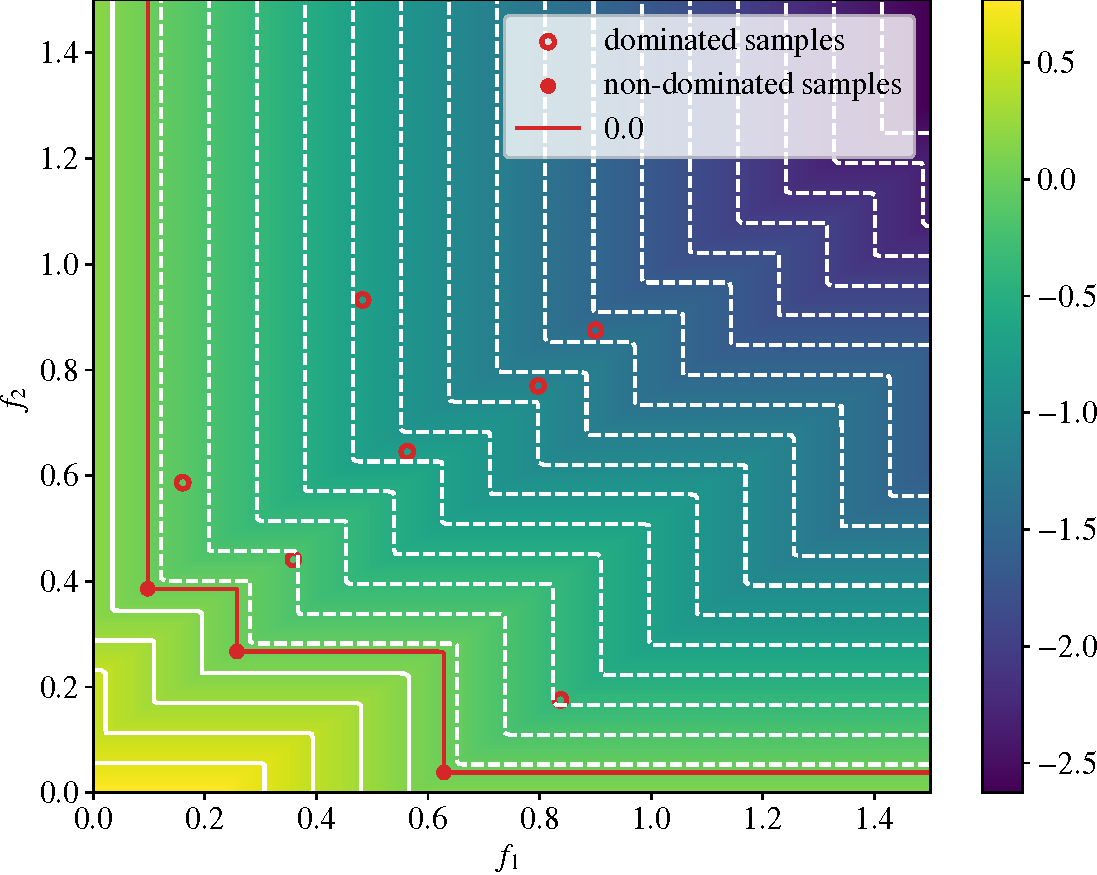
\includegraphics[width=\columnwidth]{figures/_objective_space_SAF_mu.pdf}
    \caption{\safmu}
    \label{fig: saf_obj_space}
\end{subfigure}
\begin{subfigure}[t]{0.48\columnwidth}
    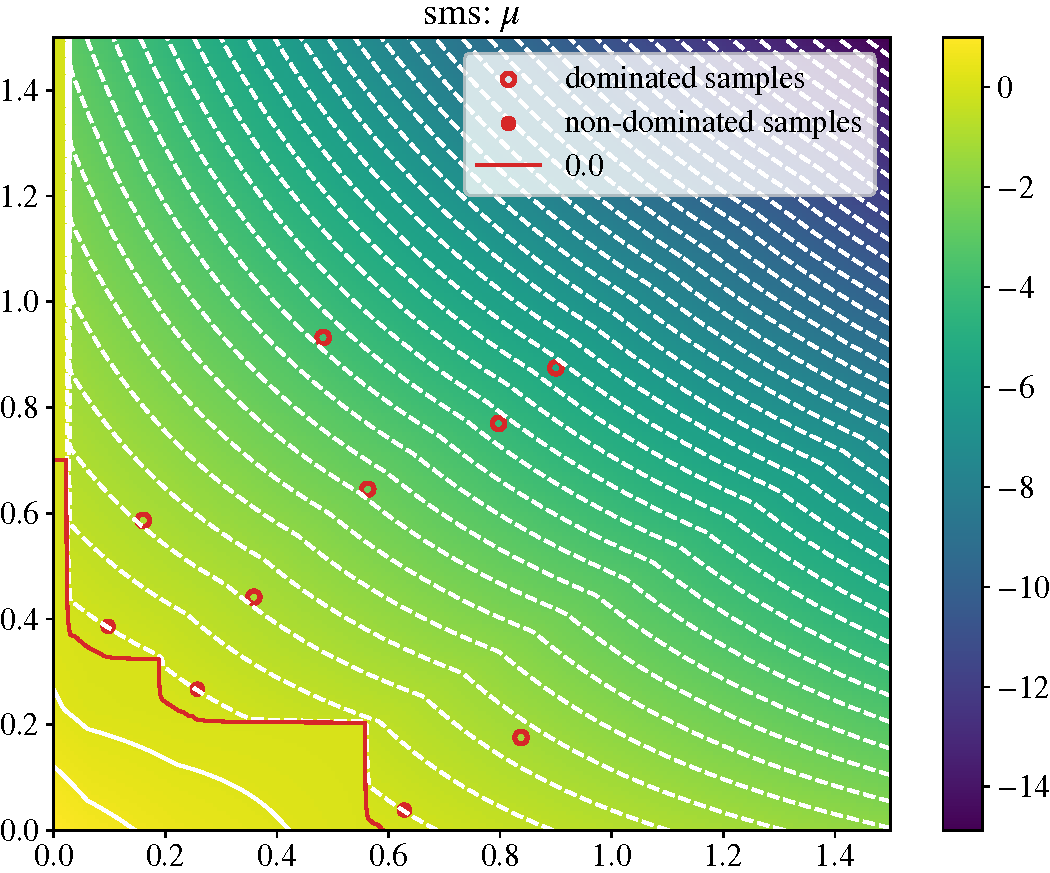
\includegraphics[width=\columnwidth]{figures/_objective_space_SMSEGO.pdf}
    \caption{\smsego}
    \label{fig: smsego_obj_space}
\end{subfigure}
\caption{
    Visualisation of infill criteria of a two objective problem,
    $\nobj=2$. The color scale shows the value of the \safmu infill criterion (left)
    and the \smsego infill criterion (right) based on the set of points
    shown, of which 3 are not dominated and form $\Fapprox$. The red curve shows contour where the
    infill criterion is zero and for \safmu corresponds to the attainment front
    $\attainmentfront_{\Fapprox}$. 
 A uniform uncertainly of $\sigma=0.05$ has been applied to the \smsego predictions, with $\epsilon=[0.058, 0.058]$ and a reference point for the hypervolume computation of $\rp=(2, 2)$.
 }
\label{fig: obj_space_comp}
\end{figure}


Similarly to Svenson and
Santer \cite{svenson2016multiobjective}  we measure the quality of a solution $\bff'$ in relation to the current approximation to the Pareto front $ \Papprox = \nondom( \data )$ as the maximin distance of $\bff'$ to the summary attainment front.  The attainment front $\attainmentfront_{\mathcal{F}}$ corresponding to a set of mutually non-dominating points $\mathcal{F}$ is a conservative interpolation of the elements of $\mathcal{F}$ so that every element of $\attainmentfront_{\mathcal{F}}$ is weakly dominated by an element of $\mathcal{F}$. More formally, the attainment front is the boundary of the region in objective space which is dominated by the elements of $\mathcal{F}$.  If
$\bu, \bv \in \reals^\nobj,$ we say that $\bu$ \textit{properly dominates} $\bv$
(denoted $\bu \lhd \bv$) iff $u_i < v_i ~\forall i = 1,\ldots, \nobj$.  Then if
\begin{align}
  \label{eq:FandU}
  \mathcal{H} &= \{\by \given \bu \prec \by \text{ for some } \bu\in \mathcal{F}\}\\
  \mathcal{U} &= \{\by \given \bu \lhd \by \text{ for some } \bu\in \mathcal{F} \}
\end{align}
the attainment front is $\attainmentfront_{\mathcal{F}} = \mathcal{H}\setminus\mathcal{U}=\partial\mathcal{U}$ \cite{smith2004dominance}.   Let $\Fapprox = \{ \bff(\bx) \given \bx \in \Papprox \}$ be the approximate Pareto front corresponding to the evaluations of $\bff$.   Then the summary attainment front infill criterion is defined as:
\begin{equation}\label{eqn: SAF}
  \saf(\by, \Fapprox) =
  \max_{i=1,\ldots, \nobj} \min_{\by' \in \Fapprox } 
  \left(
    y_i - y_i'
  \right).
\end{equation}
An image of the resultant SAF  distance generated by 3 non-dominated locations  in a two-dimensional  objective space  is shown in Fig.~\ref{fig: saf_obj_space}.   The attainment front $\attainmentfront_{\Fapprox}$ is shown in red and corresponds to the $\saf(\by, \Fapprox) = 0$ contour. The SAF infill criterion is positive behind $ \Fapprox$ (\ie for locations dominated by $\Fapprox$) and negative in front of $\Fapprox$. The figure also shows the infill criterion corresponding to SMS-EGO, which depends on the dominated hypervolume.    As can be seen, the two share broadly similar characteristics, although the infill criterion derived from the hypervolume is smoother.  We note however, that the hypervolume is much more expensive to calculate and scales poorly with the number of objectives. 
 

% Wagner \textit{et al.} \cite{wagner2010expected} lay out four specific, desirable qualities of an infill criteria as follows:
% \begin{enumerate}[label=D\arabic*:]
% \item
% For small posterior uncertainty in relation to the range of $\paretofront$, a solution should be preferred whose $\bff(\bx)$ improves the distribution and/or spread of $\paretofront$.

% \item
% Discontinuities and non-differentiabilities of the criterion should be avoided, particularly if gradient-based methods are used for the internal optimization.

% \item
% The fitness landscape of the criterion should guide the optimizer to its global optimum, e. g., plateaus should be avoided and basin sizes should grow with the quality of the corresponding local optimum.

% \item
%   The criterion should be easy to implement and efficient to calculate.
% \end{enumerate}
% The $\saf$ distance measure ensures that observations which fall in the region between two points in $\Fapprox$, in the region that is neither dominated by, nor dominates any point in $\Fapprox$, are viewed as preferable observations, even if their  distance to the ideal observation (the origin) is equivalent.\mnotejf{equivalent to what? Preferable to what?} This ensures D1 is satisfied.\rmenote{I don't understand the logic here}  D2 is also satisfied, due to the continuous nature of the distance measure in each individual objective, and the simple additive combination of objective distances. The smooth-continuous gradient towards the ideal solution, without plateaus or basins, satisfying \textit{D3}. The SAF criterion is computationally easy and cheap, much more so than the hypervolume computation required to produce \smsego, and increases linearly with the number of objectives and the size of the approximate Pareto front.

\begin{algorithm}[t!]
  \SetAlgoLined
  \KwResult{Approximation to the Pareto set for $\bff(\mathbf{x})$}
  \SetKwInOut{Input}{Input}
  \SetKwInOut{Output}{output}
  \SetKwComment{tcc}{}{}
  \SetCommentSty{textit}
  \DontPrintSemicolon
  \Input{$\ninitialevaluations$ - number of initial evaluations}
  \Input{$\nbudget$ - evaluation budget}
  \BlankLine
  %\textbf{Initialization}
  %\tcc*[l]{\textbf{Initialisation:}\hfill Generate initial samples}
  $X \gets \text{LHS}(\parameterspace, \ninitialevaluations)$ \label{alg: DSAF_LHS}
  \algremark{Generate initial samples}
  \For {$t = 1 \xrightarrow{} \ninitialevaluations$ \do}{ \label{alg:initial-start_DSAF}
    $\bff_t \gets \bff(\bx_t)$ \algremark{Expensively evaluate initial samples}
  } \label{alg:initial-end_DSAF}
  $\data  \gets \{(\bx_t, \bff_t)\}_{t=1}^{\ninitialevaluations}${\label{alg:inital-evals}}
  \BlankLine
  
 \For{$t = \ninitialevaluations+1\xrightarrow{}\nbudget$ \do}{
 \For{$j=1\xrightarrow{}\nobj$ \do}{
    $\theta_j \gets \text{train} \;\mathcal{GP}(\data)$\algremark{Train GP for each objective \label{alg:train_gp}}
    }
    $\Papprox \gets \nondom(\data)$ \algremark{Approximate Pareto set}
    \eIf{exploitative}{. 
        $\bx_t \gets \underset{\mathbf{x}\in \parameterspace}{\argmax} \:
        \saf(\mathbf{x}, \Papprox, \theta_{1:\nobj})$ 
        \algremark{\safmu} 
        \label{alg:opt-SAFmu}
    } {
    $\bx_t \gets \underset{\mathbf{x}\in \parameterspace}{\argmax} \: \ei(\mathbf{x}, \Papprox, \theta_{1:\nobj})$
    \label{alg:opt-EI_DSAF}\algremark{\safei}
    }
    
    
    $\bff_t \gets \bff(\bx_t)$ \label{alg:expensive_DSAF} \algremark{Expensively evaluate $\bx_t$}
    $\data  \gets \data \cup \{(\bx_t, \bff_t )\}$\algremark{Augment data}
 }
 $  \Papprox \gets \nondom(\data)$ \algremark{}
 \Output{$\Papprox$}
 \caption{Multi-objective Bayesian optimisation with SAF} 
 \label{alg:ourAlg_pseudocde} 
\end{algorithm}


We compare two multi-objective Bayesian optimisation algorithms based on the SAF infill criterion.  In the first (denoted by \safei), we use the SAF infill criterion in conjunction with the expected improvement acquisition function.  
In single-objective Bayesian optimisation it has recently been suggested that purely exploitative  methods (or ones that devote very little computational resource to deliberate exploration) are preferable over those which deliberately explore more such as the \ei \cite{death2019greed}. The reason advanced for this is that exploitative methods are sufficiently \textit{fortuitously} exploitative in their nature without the need for active exploration. There work showed that deploying an exploitative, $\epsilon$-greedy' optimisation strategy was often preferable in problems where the parameter space was high-dimensional and thus the objective function complex.  For this reason, we also use the SAF infill criterion, but only use the mean posterior prediction $\bmu(\bx) = (\mu_1(\bx), \mu_2(\bx),\ldots, \mu_\nobj(\bx)\trp$ where $\mu_i(\bx)$ is given by \eqref{eqn: mu}.  We denote this algorithm by \safmu.   Use of solely the mean prediction has the computational advantage of not requiring a Monte Carlo integration to approximate the \ei. In addition we have noticed that the posterior uncertainty is often so great that model predictions are made well beyond the actual Pareto front. These predictions can carry significant weight in the \ei estimation leading to the optimisation focusing on regions, which although apparently promising, are in fact infeasible.  This effect is reduced if only the mean prediction is used.  We also note that since the posterior uncertainty is not required, a wider range of surrogates (\eg random forests, support vector machines) could be employed. 

%The multi-objective Bayesian optimisation procedure is as shown Algorithm \ref{alg:BO} with the mod


Algorithm  \ref{alg:ourAlg_pseudocde} summarises the multi-objective
optimisation procedure using $\saf$.   
Initially a series of $\ninitialevaluations$ evaluations of the objective
function are made via  Latin hypercube sampling, These initial samples are
then expensively evaluated by the objective function to produce a set of
observed function values  $\data = \{(\bx_t,
\bff_t)\}_{t=1}^{\ninitialevaluations}$ (line \ref{alg:inital-evals}).
Separate \gp surrogates are then fitted, one for each of the $\nobj$
objectives (line \ref{alg:train_gp}). Here we use the Mat{\'e}rn $5/2$ kernel (as recommended for modelling realistic functions \cite{snoek2012practical}) and the parameters of these \gps are
learned by maximising the marginal log likelihood.
 The location $\bx_t$  for the next expensive
evaluation is found by maximising either the SAF infill criterion using the mean predictions from the
surrogate model or the \ei calculated via Monte Carlo sampling from the
posterior prediction using the well-known known CMA-ES optimiser
 \cite{hansen2003reducing}; lines \ref{alg:opt-SAFmu} and \ref{alg:opt-EI_DSAF}. 
  The objective function is then evaluated at
 $\mathbf{x}_t$ and the process repeated until the evaluation budget $\nbudget$ is
 exhausted or satisfactory convergence has been obtained.  The best
 estimate of the Pareto set is, at each stage of the algorithm, the maximal
 non-dominated set of locations that have been expensively evaluated.
 










\section{Experimental evaluation}
\label{sec:exper-eval}
\subsection{Process}
In this section an analysis is conducted of the performance of \safmu over 150 evaluations of a set of challenging, synthetic MOPs. For comparison we benchmark the state-of-the-art \smsego \cite{ponweiser2008multiobjective} and the competitive, yet computationally efficient \parego \cite{knowles2006parego}. We also compare the, cheap-to-evaluate minimum probability of improvement (\mpoi) infill criterion proposed by Rahat \etal \cite{rahat2017alternative}. For \smsego we  include the later improvements to the treatment of the objective space dominated by the attainment surface described by Wagner \etal \cite{wagner2010expected}.  The prior knowledge of the objective space required to set the reference point for the hypervolume calculation is assumed to be unknown. Instead the reference point $\rp$ is updated at each evaluation to the maximum value of the function observed in each objective, plus an offset of $1$, as in the original work $R_m = \max_{\bff \in \Fapprox}(f_m) +1$. %\fnote{I dont think this is clear enough, need to show np.axrgmax($\attainmentfront$, axis=0)}. 
In order to test whether more a exploitative search will be beneficial, we also include the \ei based \maximin model proposed by Svenson and Santner  \cite{svenson2016multiobjective}, (hereby denoted as \safei), and also a version of \smsego, where the uncertainty from the \gp is ignored, instead using mean prediction only, with no correction for $\epsilon$ (denoted \smsegomu). Finally, we also compared with Latin hypercube sampling (LHS). %, these strategies are listed in table \ref{table:alg_table}\fnote{I don't think this table is really necesary. Left it in for now to gauge your opinions.}.

% \begin{table}[t]
%     \setlength{\tabcolsep}{2pt}
%     \sisetup{table-format=1.2e-1,table-number-alignment=center}
%     \resizebox{\columnwidth}{!}{%
%     \begin{tabular}{|l|l|l|}
%         \hline
%         Optimiser name & Surrogate  & Comment\\
%         \hline
%         \safei & Multi & \ei version of SAF, as proposed in \cite{svenson2016multiobjective}. \\
%         \safmu & Multi & Our proposed Optimiser. (See Alg. \ref{alg:ourAlg_pseudocde}) \\
%         \smsego& Multi & Current state-of-the-art. \cite{ponweiser2008multiobjective} \\
%         \smsegomu & Multi & Modification to current SOA to be more exploitative.\\
%         \parego & Mono & Efficient computation \cite{knowles2006parego}\\
%         \mpoi & Multi & Benchmark for EMO over infill criteria approach \cite{rahat2017alternative}. \\
%         LHS & None & Baseline comparison to pseudo-uniform sampling $\parameterspace$. \\
%         \hline
%     \end{tabular}}
%     \caption{Optimisation strategies to be compared}\label{tab1}
%     \label{table:alg_table}
% \end{table}



Each optimisation was started from 10 initial \lhs samples, over 31 repeat optimisations of each test function. To ensure comparability the repeats are structured so that the same random seed and \lhs samples are used for all optimisation methods within each repeat.  The \hpv is calculated using the Fonseca \etal  method \cite{fonseca2006improved}.

% \begin{itemize}
    % \item HOW CONDUCTED
    % \item analysis of performance on complex set of problems
    % \item to test two parts of hypothesis we test both mu and ei for saf and sms. And we compare to state of the art, efficient (Parego) and SOA SMS ego. AS well as MPOI method which has been shown to outperform other cheap infills (true?) 
    % \item over budget of 250 evaluations
    % \item 31 repeats of each optimiser
    % \item starting from 10 LHS samples
    % \item paired evaluations
    % \item where required hypervolumes calculated using Fonseca,
    % \item reference points selected from the maximum observed attainment front*1.5
    % \item GPs fitted to data scaled to std 1, mean 0. 
% \end{itemize}

The chosen objective functions for the benchmark tests are a subset the Walking Fish Group problems \cite{huband2005scalable} WFG1-WFG6, which include deceptive functions and functions in which the parameters dictating distance from, and position along the Pareto front are not separable. The dimension of the parameter-space $\ndim$ for the WFG problems is scalable, as is the number of objectives $\nobj$. We tested each function over three configurations of each problem in WFG1-WFG6, with 2, 3 and 4 objectives, and $\ndim$ ranging from 6-12 dimensions. The exception to this is WFG2, which proved difficult  for all strategies, and so had the parameter space reduced to the minimum permissible $d \in [3, 4, 5]$.  More details of the test functions can be seen in Table \ref{tab: f_table}.


\begin{table}[t]
    \setlength{\tabcolsep}{2pt}
    \sisetup{table-format=1.2e-1,table-number-alignment=center}
    \resizebox{\columnwidth}{!}{%
        \begin{tabular}{|l|r|r|r|l|}
            \hline
            Function 
            &  \multicolumn{1}{c|}{$\nobj$} 
            & \multicolumn{1}{c|}{$\parameterspace$}
            & \multicolumn{1}{c|}{$\ndim$}
            & Comment\\
            \hline
            WFG1 & 2, 3, 4 & $[0, 2d]^d$ & $3, 4, 5$ &  separable, uni-modal \\
            WFG2 & 2, 3, 4 & $[0, 2d]^d$ & $6, 6, 10$ & non-separable, multi-modal\footnotemark{}, $\paretofront$ is discontinuous. \\
            WFG3 & 2, 3, 4 & $[0, 2d]^d$ & $6, 10, 10$ &  non-separable, uni-modal \\
            WFG4 & 2, 3, 4 & $[0, 2d]^d$ & $6, 8, 8$ & separable, multi-modal\\
            WFG5 & 2, 3, 4 & $[0, 2d]^d$ & $6, 8, 10$ & separable, deceptive\\
            WFG6 & 2, 3, 4 & $[0, 2d]^d$ & $10, 6, 12$ & non-separable, uni-modal\\
            \hline
        \end{tabular}}
        \caption{Walking Fish Group test functions.}\label{tab: f_table}
\end{table}
\footnotetext{Multi-modal in only the first objective $f_{1}$, uni-modal in $f_{2} \cdots f_{\nobj}$.}

Two metrics were used to quantify the performance of each optimiser. The first was the \hpv or $\mathcal{S}$-metric measure. This is a commonly used convergence measure, but as it is also the principal quantity driving \smsego. We also compared algorithms using the   Inverted Generational Distance plus (\igd) \cite{ishibuchi2015modified} in order to identify any undue bias in favour of the \smsego and \smsegomu methods. Given a set of reference points $\pigdref$ on the true Pareto front, $\igdp$ is
\begin{equation}
    \igdp(\Fapprox, \pigdref) = \frac{1}{\abs{\pigdref}}
    \sum_{\mathbf{z}\in\pigdref} \min_{\bff \in \Fapprox} d^{+}(\bff, \mathbf{z})
\end{equation}
where $d^{+}$ is the modified Euclidean distance given by:
\begin{equation}
    d^+(\mathbf{z}, \mathbf{f}) = \sqrt{\sum^{\nobj}_{i=1}\max(f_i - z_i, 0)^2}
\end{equation}
Measurements using \igd rely on a set of reference points $\pigdref$ on the problem's Pareto front. In order to ensure no bias toward solutions found in localised regions of this surface it is important that the points be distributed evenly across the front. The nonlinearity of the objective functions means that the images of  uniformly distributed samples from the Pareto set in parameter space are not uniformly distributed on $\mF$.  In order to achieve an approximately uniform distribution, we first sampled a non-uniform, but dense population of points on this Pareto front.  We then uniformly sampled the attainment surface  using the methods described by Smith \etal \cite{smith2004dominance}. Attainment surface points which did not lie on the Pareto front were then discarded if their distance to the nearest neighbour in the set of Pareto optimal points, was greater than a certain threshold. This sampling method was used for all functions with the exception of WFG3, for which the Pareto surface is straightforward to compute and sample uniformly. Example reference points are shown in Fig. \ref{fig: refpoints_wfg4}.  

\begin{figure}[t]
\begin{subfigure}[t]{0.45\columnwidth}
    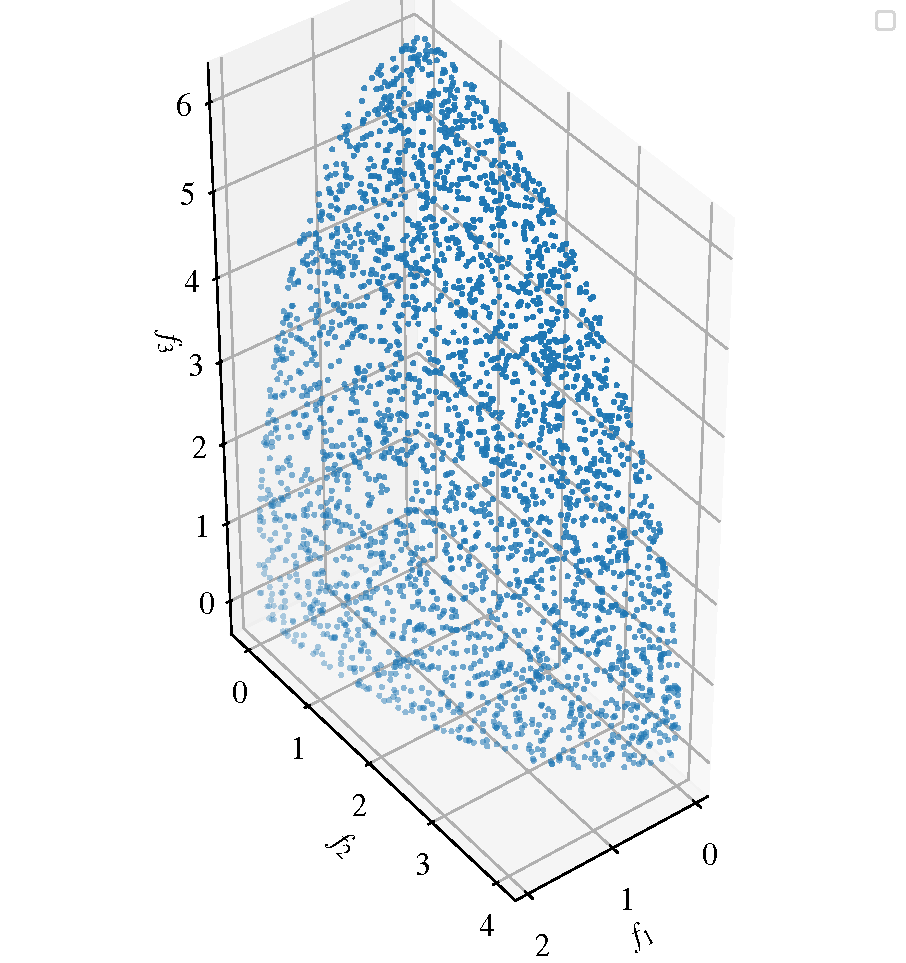
\includegraphics[width=\columnwidth]{figures/_IGD_refpoint_example_WFG4.pdf}
    \caption{WFG4, WFG5 \& WFG6}
    \label{fig: refpoints_wfg4}
\end{subfigure}
\begin{subfigure}[t]{0.45\columnwidth}
    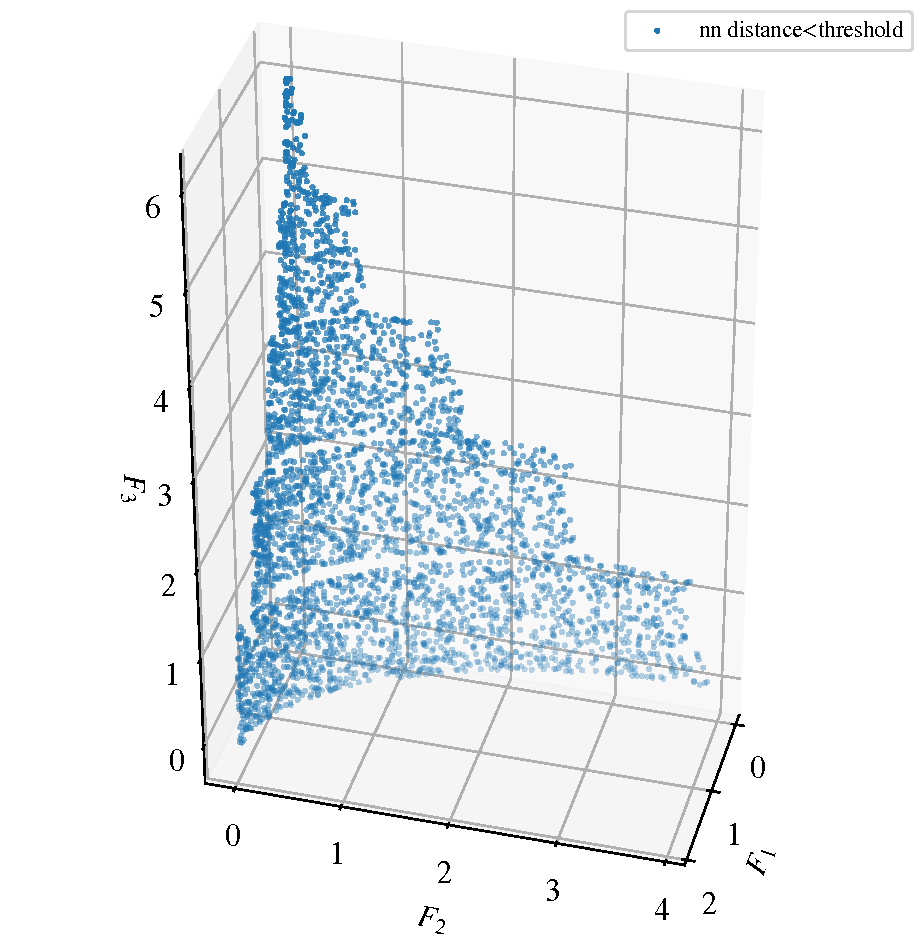
\includegraphics[width=\columnwidth]{figures/_IGD_refpoint_example_WFG2.pdf}
    \caption{WFG2}
    \label{fig: refpoints_wfg2}
\end{subfigure}
\caption{\igd reference points, for 3 objective WFG problems.}

\end{figure}

% \begin{itemize}
    % \item HOW ASSESSED
    % \item which problems chosen?
    % \item why problems chosen? build on DTLZ, include various features (multimodal, convex, separable). 
    % \item why d6? reduced dimensionality for wfg1 to facilitate finding better solutions
    % \item measurements taken using dominated hypervolume and igd+
    % \item igd+ samples taken by oversampling the pareto front, and then drawing a random sample from this using the attainment sampling techinique described in richards paper. 
    % \item results compared by their median value, with statistical equivlance tested using Holm-bonferoni corrected wilcoxen signed rank test. 
    % \item problem table
% \end{itemize}

\subsection{Results}


The results of the optimisations, as measured by \hpv and \igd, are shown in table \ref{tab: results}. These tables show the median result and interquartile range (IQR) for each optimiser over the 31 repeated runs on each test problem. The best median performance is shaded in dark grey, with any statistically similar results, as assessed by paired Wilcoxon signed-rank test\rmenote{References removed here} 
%\cite{woolson2007wilcoxon} 
with Holm-Bonferroni correction 
% \cite{holm1979simple} 
($p>0.05$) shaded in light grey.

After the  150 budgeted evaluations of the objective functions, \safmu produced either the best median \hpv performance, or was statistically equivalent to the best median performance in 12 out of the 18 tested problem configurations. This was the most out of any of the considered alternatives, with \smsego giving best or equivalent performance on 8 objective functions. The results as measured by \igd were similar, with \safmu again offering the best or equivalent performance in 12 out of 18 functions, and \smsego in 10. The sets of non-dominated solutions produced by each method were not characteristically different, and both generally produced good coverage of the Pareto front.\rmenote{Evidence for these claims?}  

As may be expected, performance of the optimisers varies between problems. The purely exploratory \lhs method was not the best optimisation strategy for any of the problems tested, and in fact was the worst performer on all problems aside from the difficult WFG2 problem. WFG2 was poorly optimised across the board, with the majority of the Pareto front left unexplored by all optimisers. While \parego and \lhs excelled here relative to their performances on other objective functions (beating \smsego, \smsegomu and \safei in the two-objective configuration), still few solutions were found in much of the objective space.\rmenote{I've commented out the WFG2 discussion as it's long and I'm not entirely convinced.  Best to stick to the mai message at first.}
\begin{comment}

It is worth noting that WFG2 is the only problem here with a discontinuous Pareto front, and also the only problem in which the boundary between the attainable and unattainable objective space regions, on which the Pareto front lies, extends into the region dominated by the Pareto optimal solutions. Therefore much of the objective space, in between the acquired evaluations, and favoured by infill criteria methods may unattainable. This is a feature which distinguishes this function from the others tested here but could be a factor in the poorer performance by optimisers reliant on infill criteria.\rmenote{I'm not entirely convinced by this} %\fnote{Not sure this makes sense. We should talk about it and see if you both think it is relevant: In all other problems, any point dominated by the current attainment set, is guaranteed to be also attainable. This is not the case for WFG2.} 
This is also the only function tested with a discontinuous Pareto front, and isolated local minima are positioned on the front in between unattainable regions. \hpv and $\igdp$ scores in the two-objective case were largely distinguished by whether or not the second local minima was found, as a solution in this second minima would greatly affect the \hpv measurement.
 
\end{comment}


\begin{table*}[t]
\begin{subtable}[t]{.49\textwidth}
\begin{subtable}[b]{\textwidth}
\setlength{\tabcolsep}{2pt}
\sisetup{table-format=1.2e-1,table-number-alignment=center}
\resizebox{\columnwidth}{!}{%
\import{tables/}{hv_table_1.tex}}
\smallskip
\end{subtable}
\begin{subtable}[b]{\textwidth}
\setlength{\tabcolsep}{2pt}
\sisetup{table-format=1.2e-1,table-number-alignment=center}
\resizebox{\columnwidth}{!}{%
\import{tables/}{hv_table_2.tex}}
\smallskip
\end{subtable}
\begin{subtable}[b]{\textwidth}
\setlength{\tabcolsep}{2pt}
\sisetup{table-format=1.2e-1,table-number-alignment=center}
\resizebox{\columnwidth}{!}{%
\import{tables/}{hv_table_3.tex}}
\end{subtable}
\end{subtable}
\hfill
\begin{subtable}[t]{0.49\textwidth}
\begin{subtable}[b]{\textwidth}
\setlength{\tabcolsep}{2pt}
\sisetup{table-format=1.2e-1,table-number-alignment=center}
\resizebox{\columnwidth}{!}{%
\import{tables/}{igd_table_1.tex}}
\smallskip
\end{subtable}
\begin{subtable}[b]{\textwidth}
\setlength{\tabcolsep}{2pt}
\sisetup{table-format=1.2e-1,table-number-alignment=center}
\resizebox{\columnwidth}{!}{%
\import{tables/}{igd_table_2.tex}}
\smallskip
\end{subtable}
\begin{subtable}[b]{\textwidth}
\setlength{\tabcolsep}{2pt}
\sisetup{table-format=1.2e-1,table-number-alignment=center}
\resizebox{\columnwidth}{!}{%
\import{tables/}{igd_table_3.tex}}
\end{subtable}
\end{subtable}

\caption{The median \hpv (left) and $\igdp$ (right) measured after 150 function evaluations and the associated interquartile ranges (IQR), over 31 repeated optimisations of the WFG test functions. The best median performance is shaded in dark grey, while performances which are statistically equivalent are shaded light grey.}
\label{tab: results}
\end{table*}


The measurements in Table \ref{tab: results} only consider a slice of the optimisation process, when the algorithms have largely converged. Figure \ref{fig: ranked_plots} shows average ranked performance over all 31 repeats and all objective functions in the experimental evaluation, at every step of the optimisation. Where the difference between optimisations of similar rank were not statistically significant (according to Wilcoxon signed-rank test) the two were assigned the mid-point between their respective ranks. From this it is  clearer that over the full  range of test problems \safmu shows the  best overall performance in the final stages whether measuring by $\igdp$ or \hpv, but also shows competitive performance throughout the process. \smsego and \smsegomu rank similarly and competitively with \safmu, but \safei falls well behind after a few initial, favourable evaluations. This is surprising as one might expect \safei to find better solutions in the later stages, when a more complete representation of the optimised function has been formed by the surrogate \cite{death2019greed}. However, we speculate that even after 150 evaluations the surrogate is insufficiently faithful that deliberate exploratory evaluations are required. 

Neither \mpoi or \safei, which account for the surrogate's uncertainty, are competitive over the broad range of functions tested, with both falling well short of the exploitative \safmu approach in the majority of functions tested. In problems where \safei failed to match the results obtained by \safmu the solutions found were similar, but there were far fewer non-dominated solutions produced after 150 evaluations; for example, \safei, finds an average of 98 non-dominated in $\text{WFG}5$ ($\nobj = 3$ and $\ndim = 8$) compared to 128 found by \safmu.

\begin{figure}[t]
\begin{subfigure}[b]{\columnwidth}
         \centering
         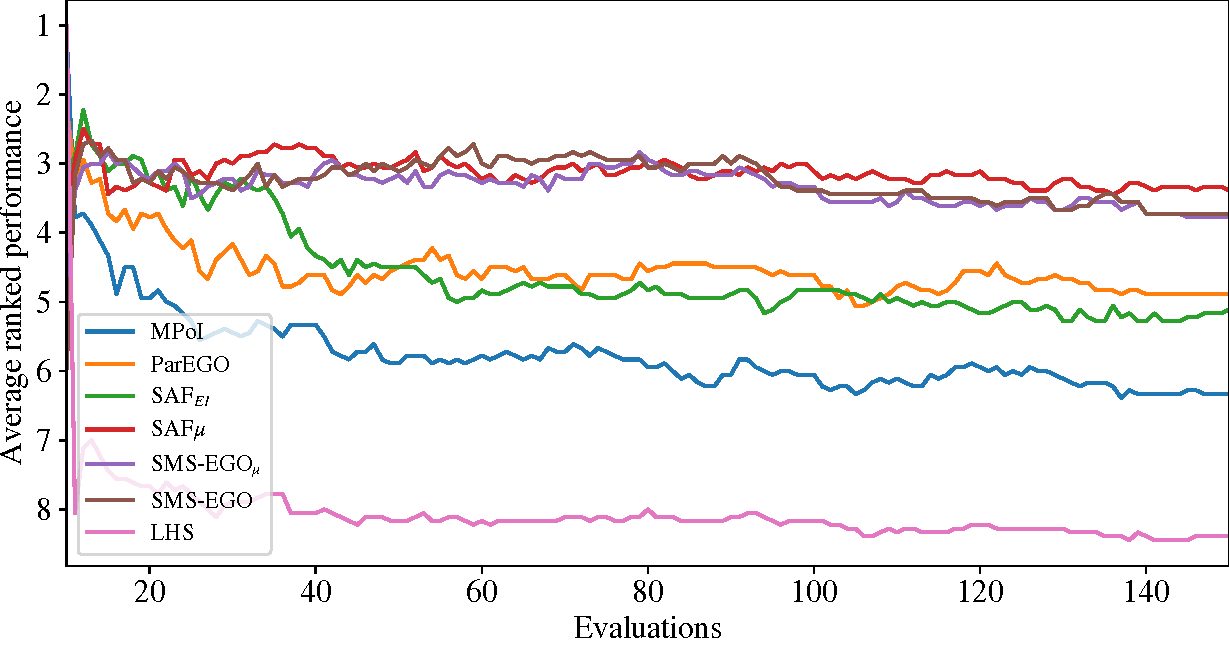
\includegraphics[width=\columnwidth]{figures/_ranked_performance_plot_hv.pdf}
        %  \label{fig: ranked_hv_plot}
     \end{subfigure}
\begin{subfigure}[b]{\columnwidth}
         \centering
         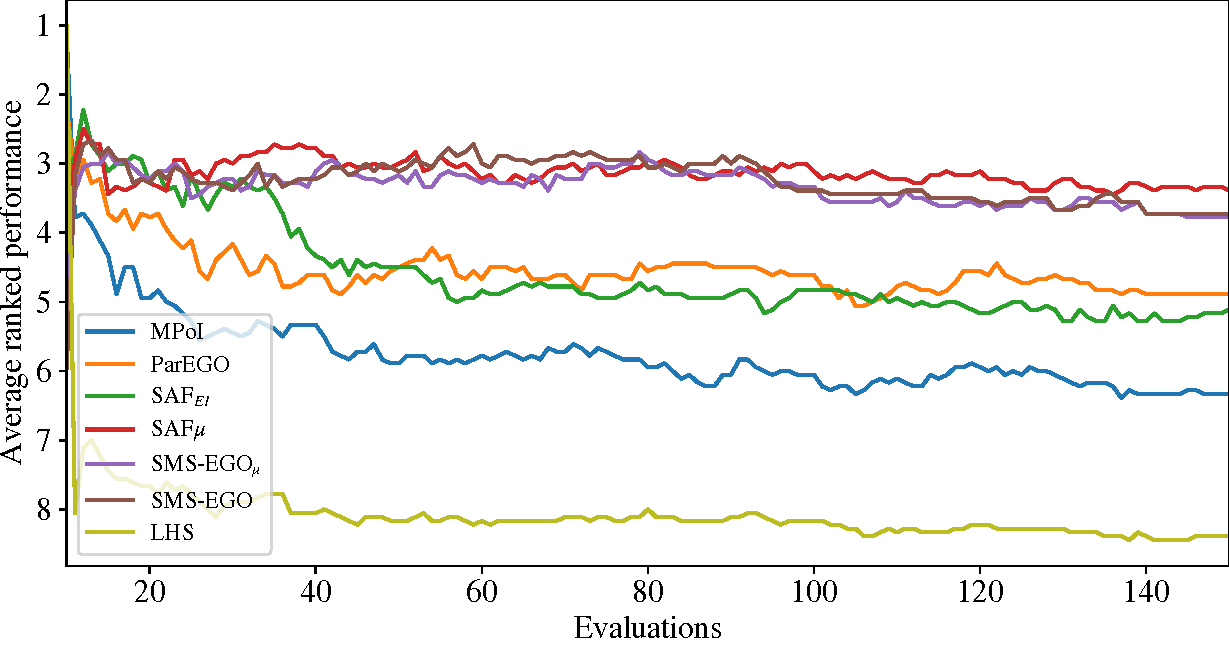
\includegraphics[width=\columnwidth]{figures/_ranked_performance_plot_igd.pdf}
        %  \label{fig: ranked_igf_plot}
     \end{subfigure}
\caption{Average ranked performance of each optimiser, as measured by \hpv (above) and $\igdp$ (below).}
\label{fig: ranked_plots}
\end{figure}



As measured by \hpv \safmu is never surpassed in a statistically significant manner by any of the computationally inexpensive alternatives (\lhs, \mpoi, \parego \& \safei), with the exception of two of the poorly optimised WFG2 benchmarks. \safmu is also better when measured by \igd in the vast majority of cases, and its average ranked performance is  better than any of these methods beyond the initial 10 steps of the optimisation, whichever measurement method is used (Figure \ref{fig: ranked_plots}).  



The two methods which utilise hypervolume calculations in their infill criteria, \smsego and \smsegomu, did not demonstrate better overall performance than the cheap \safmu method. Nor did the posterior uncertainty information leveraged by \smsego benefit it significantly over \smsegomu. \smsego had slightly more \textit{winning} results, being the best or equivalent in 10 out of 18 experiments compared to 8 by \smsegomu when measured by \hpv (both with 10 by \igd), but the average ranked performances were very similar. \smsego represents the state of the art, and was inferior in the majority functions tested in this set of experiments to the proposed \safmu method. 

\begin{figure}[t]
         \centering
         %\fbox
         \label{fig: exemplar_pf_sms_saf_hv}
\caption{Convergence of tested algorithms on WFG5 ($\nobj = 3,$ $\ndim = 8$) over 150 evaluations, starting from 10 LHS samples. Solid lines show median values over 31 repeats and shaded regions show the IQR.}
\label{fig: exemplar_pf}
\end{figure}


\section{Conclusion}\label{sec:conclusion}
When optimising expensive, multi-objective problems efficient use of objective evaluations is critical to convergence within the constraining budget. Current state-of-the-art methods for optimising such problems in few evaluations rely on \hpv based infill criteria, which can themselves become prohibitively costly as the number of objectives is grows, and the number of solutions increases. 

\rmenote{I think the conclusions should be about (a) Cheap calculation of SAF compared with SMS-EGO and (b) No need for deliberately exploratory evaluations (c) GPs not needed and others e.g. RFs or SVMs could be used.}A novel infill criterion is presented, producing state-of-the-art results, with low computational complexity, and without requiring \hpv computation. Our method is benchmarked against current leading methods, shown to be similarly effective over the problems tested to the state of the art, and shown to surpasses the leading low-complexity alternatives in the majority of objectives tested. 

We further show that in multi-objective optimisation, exploiting the mean prediction of the surrogate model is more often than not superior to leveraging the posterior prediction uncertainty in order to deliberate exploration of the objective space. This presents an opportunity to broaden the scope of surrogate models used in Bayesian optimisation to those which may be able to better model complex objective functions, but do not provide uncertainty estimates for posterior prediction. 


% \section{Definitions required}
% \begin{enumerate}
%     \item Objective space
%     \item Domination
% \end{enumerate}


% \section{Consideratios/ammendments to be made}
% \begin{itemize}
%     \item hyphenate multisurrogate, monosurrogate, single surrogate
%     \item check for consistency in parameters vs inputs, 
%     \item Do i need to explain traingp in algorithms?
%     \item MOOP vs MOP vs MOO<- pick one
%     \item define HV
%     \item state of the art vs state-of-the-art
%     \item check  S-metric
% \end{itemize}
\bibliographystyle{ieeetr}
\bibliography{bibliography}

\end{document}

%%% Local Variables:
%%% mode: latex
%%% TeX-master: t
%%% End:

